\documentclass{standalone}
\usepackage{tikz}
\usepackage{float}
\usepackage{amsmath}
\usepackage{lmodern}
\usepackage{amssymb}
\usepackage{pgfplots}
\usetikzlibrary{calc}
\usetikzlibrary{hobby}
\usepackage{nicefrac}
\usetikzlibrary{decorations.markings}
\usetikzlibrary{patterns, patterns.meta}
\usetikzlibrary{shapes}
\usetikzlibrary{shapes.misc}
\pgfplotsset{compat=1.18}
\begin{document}
\centering

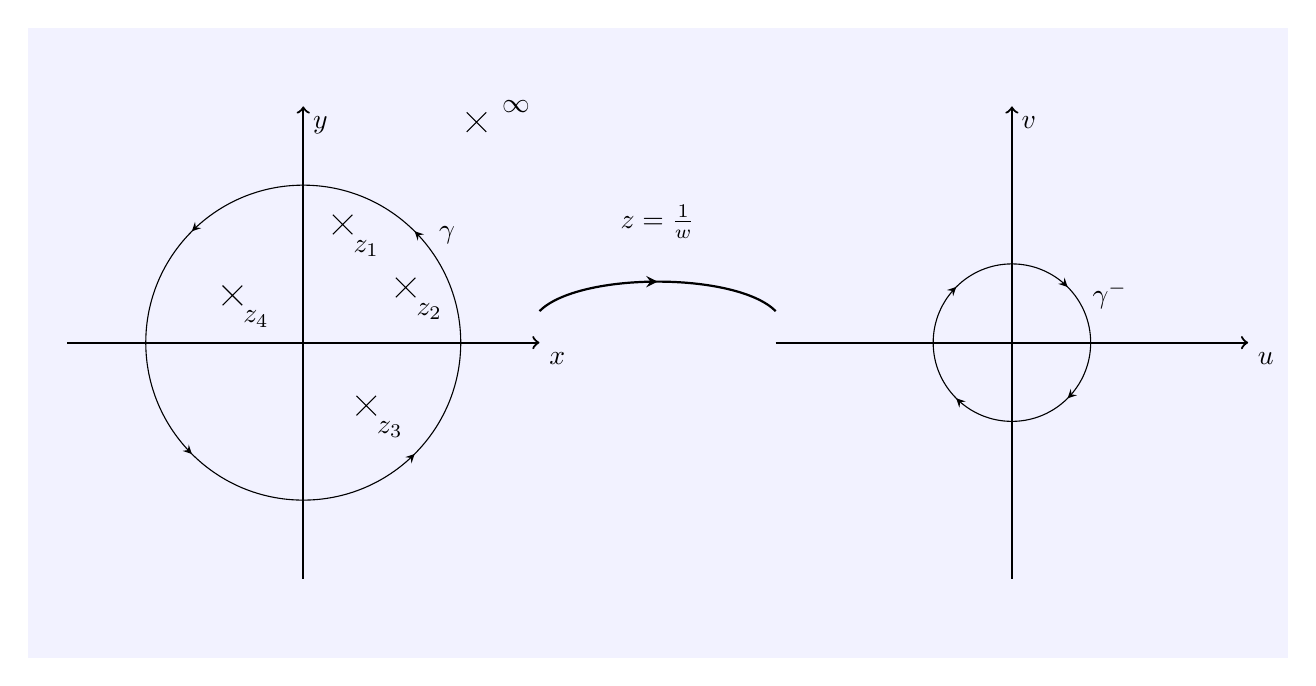
\begin{tikzpicture}
    % Background for entire canvas
    \fill[blue!5] (-8,-4) rectangle (8,4);

    % === Figure positions ===
    % We'll define each figure in its own scope with a shift

    %gladde kromme er tussen

    \draw[thick,postaction={decorate}, decoration={markings,mark=at position 0.5 with {\arrow{stealth}}}][black] (-1.5,0.4)
    .. controls (-1,0.9) and (1,0.9) .. (1.5,0.4);
    \node[above] at (0,1.2) {$z=\frac{1}{w} $};

    
    % ----------------------
    % First Figure
    \begin{scope}[shift={(-4.5,0)}]
    % Assen
    \draw[thick, ->] ($(-3,0)$) -- ($(3,0)$);
    \draw[thick, ->] ($(0,-3)$) -- ($(0,3)$);
    \coordinate (x) at (3,0);
    \draw (x) node[below right] {$x$};
    \coordinate (y) at (0,3);
    \draw (y) node[below right] {$y$};
    % Cirkel
    \draw[postaction={decorate}, decoration={markings,mark=at position 0.125 with {\arrow{stealth}},mark=at position 0.375 with {\arrow{stealth}},mark=at position 0.625 with {\arrow{stealth}},mark=at position 0.875 with {\arrow{stealth}}}](2,0) arc[start angle=0, end angle=360, radius=2];
    \coordinate (G) at (1.6,1.6);
    \draw (G) node[below right] {$\gamma$};
    \coordinate (inf) at (2.4,3.2);
    \draw (inf) node[below right] {$\infty$};
    %draw poles
    \node[solid, cross out,draw=black] at (2.2,2.8) {};

    %draw poles
    \node[solid, cross out,draw=black] at (0.5,1.5) {};
    \node at (0.8,1.2) {\textcolor{black}{$z_1$}};
    \node[solid, cross out,draw=black] at (1.3,0.7) {};
    \node at (1.6,0.4) {\textcolor{black}{$z_2$}};
    \node[solid, cross out,draw=black] at (0.8,-0.8) {};
    \node at (1.1,-1.1) {\textcolor{black}{$z_3$}};
    \node[solid, cross out,draw=black] at (-0.9,0.6) {};
    \node at (-0.6,0.3) {\textcolor{black}{$z_4$}};

    \end{scope}



    
    \begin{scope}[shift={(4.5,0)}]
    % Assen
    \draw[thick, ->] ($(-3,0)$) -- ($(3,0)$);
    \draw[thick, ->] ($(0,-3)$) -- ($(0,3)$);
    \coordinate (u) at (3,0);
    \draw (u) node[below right] {$u$};
    \coordinate (v) at (0,3);
    \draw (v) node[below right] {$v$};
    % Cirkel
    \draw[postaction={decorate}, decoration={markings,mark=at position 0.125 with {\arrow{stealth}},mark=at position 0.375 with {\arrow{stealth}},mark=at position 0.625 with {\arrow{stealth}},mark=at position 0.875 with {\arrow{stealth}}}](1,0) arc[start angle=0, end angle=-360, radius=1];
    \coordinate (W) at (0.9,0.9);
    \draw (W) node[below right] {$\gamma^-$};    
    \end{scope}
\end{tikzpicture}
\end{document}